\section{Plant as sensor}

%TODO: Write an introduction

\subsection{Technical choices}

%TODO: Rework the technical choices part.
Before diving into the implementation, several technical choices were made to shape the overall design of the system. The first major decision was selecting the ESP32 microcontroller as the core processing unit due to its versatility, offering built-in WiFi, multiple GPIO pins, and analog-to-digital converters, which allow for handling sensor data and wireless communication efficiently.

Additionally, the system's audio capabilities were a critical consideration, leading to the inclusion of a basic amplification circuit to boost sound output, ensuring compatibility with external speakers. The design also included a micro-SD slot to allow for expandable storage, enabling future enhancements like storing pre-recorded sounds or more detailed data logs. These foundational decisions laid the groundwork for a scalable and reliable system, ensuring smooth integration of the components that follow in the implementation.

\subsection{The electronic interface}

The electronic interface is the interface that allows a compute unit to capture and interpret the plant signal and
communication. The interface is a device made by us for this use case. The printed circuit board (PCB)
device is composed of 3 main parts:
\begin{itemize}
    \item The core of the circuit, the microcontroller, an ESP32 Wroom 32
    \item An electronic filter connected using an electrode to the plant
    \item A sound part of the PCB that is including an audio amplifier, a volume knob and a terminal block to connect a speaker
\end{itemize}

The design of the PCB has been done using the open source software Kicad.
As said previously, the circuit contains 3 parts.

The core of the circuit is the computation part, including the microcontroller, an ESP32. All the other
devices of the circuit are connected to the ESP32. The choice to use a devkit has been done
to ease the electronic conception and to avoid any communication and soldering issue with the MCU\footnote[1]{Microcontroller Unit}.

\begin{figure}[h!]
    \centering
    \includegraphics[width=\textwidth]{images/iop.pdf}
    \caption{The main schematic of the device. This main schematic regroups components and sub-sheets (including the audio circuit
        and the filter circuit). The main component is an ESP32 Wroom DevKit. All other components are linked to this
        microcontroller}
    \vspace{0.1cm}
    \label{fig:iop_schematic_main}
\end{figure}


The PCB also includes a dedicated slot for a capacitive humidity sensor (ref figure \ref{fig:moisture_sensor}). This humidity sensor is added to reinforced the data captured by the main sensor/filter. This sensor captures the moisture level in the plant's soil, providing valuable insight into the plant's overall health and hydration status.

By integrating this additional sensor, the system can monitor environmental factors alongside the main sensor's data, such as the plant's response to touch or other interactions. The humidity data complements the primary sensor readings which can be used to refine the interaction model or influence the sonification process. This added layer of data could permits more precision and complexity when doing the sonification process.

\begin{figure}[h]
    \centering
    \includegraphics[width=0.8\textwidth]{moisture_sensor.jpg}
    \caption{The sensor chosen is the capacitive moisture sensor from Seeed Studio: The Grove. This sensor is able to capture the moisture level in the plant's soil, providing valuable insight into the plant's overall health and hydration status. However, the connector on the PCB allows to connect any other sensor that has 3 pins (VCC, GND, DATA) connection.}
    \vspace{0.1cm}
    \label{fig:moisture_sensor}
\end{figure}


The circuit component that allows us to read data from the plant is the electronic filter.
This filter has been designed by \textit{Jakub Nikonowicz} and \textit{Łukasz Matuszewski}
from \textit{Politechnika Poznańska}.
Thanks to them, I adapted it for my application on my embedded device.

\begin{figure}[H]
    \centering
    \includegraphics[width=\textwidth]{images/iop-plant_filter.pdf}
    \caption{The electronic circuit designed to capture the interaction by analyzing the electronic
        frequency response. The circuit includes 3 resistors, 3 inductors and 3 capacitors as main components}
    \vspace{0.1cm}
    \label{fig:iop_schematic_filter}
\end{figure}

This filter is ending by a crocodile clamp that is directly connected to the plant.

The last part of the circuit is the sound output/rendering. This circuit includes a small amplifier,
the LM386 from Texas Instruments. The rest of the circuit are components needed in order to
induce amplification on the signal without creating to many noise and saturation.

\begin{figure}[H]
    \centering
    \includegraphics[width=\textwidth]{images/iop-audio_circuit.pdf}
    \caption{The sound output part of the circuit that is used to render the sound.
        This part includes a small amplifier, the LM386. The circuit also includes the components necessary
        to control and handle the amplification (reduce noise and saturation)}
    \vspace{0.1cm}
    \label{fig:iop_schematic_audio}
\end{figure}

The PCB is built to be able to add a micro-SD slot (ref to \ref{fig:iop_schematic_main}). This micro-SD slot
allows to increase the storage of the embedded ROM. This can be used to store pre-built sounds and music to avoid generating a sound on-board.


Once the schematic was completed, the next step was routing the tracks. There are several methods for PCB routing, including single-sided, double-sided, and multiple-layer designs. We opted for a double-sided PCB on each side because this configuration simplifies component placement, making the layout more efficient and organized. Additionally, it is significantly more cost-effective compared to multi-layer PCBs, striking a good balance between performance and budget. Indeed, in terms of routing, PCBs can be single-sided, double-sided, or multi-layered. Single-sided boards are simple and low-cost but limited in complexity. Double-sided PCBs, with copper on both sides, allow for more efficient routing and are commonly used for moderate complexity. Multi-layered PCBs offer even greater routing density, suitable for advanced electronics such as computer motherboards or phone components.

In terms of track width, we used 0.2mm wide tracks for data signals to maintain signal integrity, while the power tracks were designed with a width of 0.8mm. This wider width ensures that the power tracks can safely handle up to 800 mA, providing sufficient current capacity without overheating or voltage drops.

\begin{figure}[H]
    \centering
    \includegraphics[width=\textwidth]{images/iop-routed_pcb.pdf}
    \caption{Double sided PCB routed. This view allows to see the track used for components inter-connection. The tracks width is 0.2mm for data tracks and 0.8mm for power tracks.}
    \vspace{0.1cm}
    \label{fig:iop_routed_pcb}
\end{figure}

Kicad also allows us to generated a 3D view of the future PCB. This allows us to imagine what the
PCB will look like when it will be manufactured.
\begin{figure}[H]
    \centering
    \includegraphics[width=0.8\textwidth]{images/front_iop_3D_view_modified.png}
    \caption{Front 3D rendering of the built PCB. The rendering is done using open source software: Kicad}
    \vspace{0.1cm}
    \label{fig:front_iop_3D_view_modified}
\end{figure}

\subsection{Human interaction}

\subsubsection{Use of the sensor/filter}

The device is able to capture the human interaction with the plant. The touch interaction is inducing changes
in the impedance, capacitance and inductance of the plant. Values are captured using the GPIO (General Port Input/Output)
14 of the ESP32 DevKit. This GPIO is able to read analog data and convert them to digital values using analog to digital
converter (ADC). The values are a floating point number between %TODO: Add the range of the values here.
Values are fluctuating depending on the interaction.

%TODO: Add a table comparing the values depending on the interaction

The possibilities of


\subsubsection{Sonification on the device} % FIXME: subsubsection ??

The human interaction goes through the sonification on the device. ESP32 embeds a 8-bit digital to analog converter (DAC).
The embed DAC is enough to play low quality sounds. Combined with the micro-SD card including in it, it is a media player.
Using the \textit{Arduino Audio Tools} library it is possible to read MP3, Wav and other audio format.
Taking the sensor value as an input, you can then apply a pitch shift on the data that will be rendered on the DAC.
The pitch shift is a value included between 0 and 100. We are mapping the max value of the sensor and the min value
to this range using the \textit{map()} Arduino function.

The data is sent to the DAC and rendered. \textit{Arduino Audio Tools} also includes a way to communicate data to the
DAC.

%TODO: Add oscilloscope screenshot of the sound output.

There are two DAC available on the ESP32. DAC 1 and DAC 2 respectively on GPIO25 and GPIO26. The IoP device allows
to choose between the one you want by using a removable jumper.

The output of the DAC is too low to be able to render it on a speaker. The amplification circuit allows a small
amplification of the output. The amplifier is a basic and simple one. I added a 10k Ohms potentiometer to be able to
tweak the volume. The sound quickly reach amplifier limitations and is becoming saturated.

The amplified output is sent to a terminal block that acts as the connection interface to the audio speaker.
The audio speaker chosen in our specific example is a 8 Ohms 3 Watts speaker.

\begin{figure}[h!]
    \centering
    \includegraphics[width=0.6\textwidth]{images/speaker.jpg}
    \caption{8 ohms 3 Watts basic speaker used in our example.}
    \vspace{0.1cm}
    \label{fig:speaker}
\end{figure}


\newpage
\subsubsection{User study}
In the context of the Internet of Things (IoT), this study delves into the nascent field of human-plant interaction, as envisioned by the Internet of Plant project. 
This innovative initiative explores the potential intersections between human actions and botanical entities to create a symbiotic relationship between nature and technology. 
The central inquiry involves imagining a future where plants respond acoustically to physical touch. 
Three distinct plant species—Dypsis lutescens, Pachira glabra, and Dracaena—are employed as subjects to examine user perceptions and interactions within this imagined framework. 
The objective is to contribute to the discourse surrounding the integration of technology and nature by discerning the various ways in which individuals conceptualize and interact with plants as potential musical collaborators.


\subsu{Methodology}

\subsection{Participants}




\subsection{Procedure}

The procedure unfolded in a systematic fashion to facilitate a comprehensive exploration of participants' perceptions and interactions with the envisioned musical plants. Upon welcoming each participant, we presented them with the intriguing premise: "We're in the very near future. You are looking at plants that make music when you physically interact with them (it is not actually the case, but imagine it). Explore their capabilities." This imaginative prompt aimed to elicit uninhibited responses and creative engagement. Subsequently, participants were given the freedom to explore the potential musical capacities of the plants at their own pace. An important aspect of the procedure was our deliberate decision not to provide any guidance or answer questions during the exploration phase, allowing for unfiltered and spontaneous reactions. In instances where participants encountered difficulty initiating exploration, the prompt was reiterated to encourage a more immersive and uninhibited interaction with the conceptualized musical flora. This methodological approach was designed to capture the unmediated and diverse responses of participants as they navigated the uncharted territory of human-plant interaction. Also, we avoided any kind of communication or talking between 2 participants to reduce the potential bias.


\subsection{Materials/Tools}

To proceed and conduct this user study, we choose 3 different plants from 3 different species.

\newpage

\subsubsection{Dracaena}
They project was initially conducted using this specific plant. It has long leaves and fragile perceived trunk but also flexible.

\begin{figure}[h!]
    \centering
    \includegraphics[width=0.42\textwidth, angle=-90]{small_plant.jpg}
    \caption{The N°1 plant is a \textit{Dracaena}.}
    
    \vspace{-0.5cm}
    \label{fig:small_plant}
    \vspace{0.2cm}
\end{figure}




\subsubsection{Pachira glabra}

We chose to use this plant for its large leaves and its wide trunk. This \textit{Pachira} is a bit taller than the \textit{Dracaena} (figure \ref{fig:small_plant}).
\begin{figure}[h!]
    \centering
    \includegraphics[width=0.42\textwidth, angle=-90]{tall_plant_cropped.jpg}
    \caption{The N°2 plant is a \textit{Pachira glabra}.}
    
    \vspace{-0.5cm}
    \label{fig:tall_plant}
    \vspace{0.2cm}
\end{figure}


\newpage

\subsubsection{Dypsis lutescens}

The \textit{Dypsis lutescens} is very different from the two other plants. Indeed, it is composed of many trunks and stems. On top of that, the leaves are numerous and tight.

\begin{figure}[h!]
    \centering
    \includegraphics[width=0.42\textwidth, angle=-90]{fougere_plant.jpg}
    \caption{The N°3 plant is a \textit{Dypsis lutescens}.}
    
    \vspace{-0.5cm}
    \label{fig:fougere_plant}
    \vspace{0.2cm}
\end{figure}



\subsubsection{The experimental space}

The experimental space served as an open canvas for the exploration of human-plant interaction within the Internet of Plant project. While the configuration was not explicitly tailored to the plants, it provided a versatile environment that accommodated the envisioned musical flora. The space featured three distinct levels of height, each corresponding to one of the three plants introduced to participants. 

\begin{figure}[h]
    \centering
    \includegraphics[width=0.42\textwidth]{setup_user_study.jpg}
    \caption{User study space setup. The setup is built from our lab space.}
    
    \vspace{-0.5cm}
    \label{fig:setup_user_study}
    \vspace{0.2cm}
\end{figure}

\section{Data collection}
To capture the nuances of participant interactions with the conceptualized musical plants, a collaborative approach was adopted, involving two researchers to provide dual perspectives. Throughout the exploration phase, both researchers meticulously took notes, documenting the diverse ways in which participants engaged with the three distinct plants. Each note explicitly specified the plant involved in the interaction, ensuring a granular understanding of the responses tied to each botanical entity.

The notes encompassed detailed descriptions of participants' actions, expressions, and verbalizations, aiming to encapsulate the richness of their experiences. The dual-observer strategy facilitated a more comprehensive and triangulated perspective, mitigating potential biases and enhancing the reliability of the recorded data. The collaborative note-taking process served as a valuable means of capturing the multifaceted nature of human-plant interaction within the experimental context, contributing to the depth and richness of the findings in the subsequent analysis.

We defined 5 possible interaction :

\begin{itemize}
    \item Grasp : user uses the whole hand to grab trunk or leaves
    \item Pinch : user uses 2 to 3 digits to grab trunk or leaves
    \item Slide : user uses his/her hand or finger to slide on the plant
    \item Pet : user uses his/her hand to cuddle the plant or to pass through the leaves
    \item Tam Tam : user taps on the plant mainly using the whole hand
\end{itemize}


\section{Results}
Looking at the results, we extracted the table \ref{tab:results}.


\begin{table}[ht]
\begin{tabular}{|l|ll|l|ll|}
\hline
\multirow{2}{*}{Plant/Interaction} & \multicolumn{2}{l|}{Group 1}       & Group 2 & \multicolumn{2}{l|}{Group 3}       \\ \cline{2-6} 
                                   & \multicolumn{1}{l|}{Grasp} & Pinch & Slide   & \multicolumn{1}{l|}{Pet} & Tam Tam \\ \hline
Plant N°1                          & \multicolumn{1}{l|}{4}     & 8     & 4       & \multicolumn{1}{l|}{4}   & 2       \\ \hline
Plant N°2                          & \multicolumn{1}{l|}{9}     & 3     & 3       & \multicolumn{1}{l|}{3}   & 10      \\ \hline
Plant N°3                          & \multicolumn{1}{l|}{10}    & 1     & 5       & \multicolumn{1}{l|}{7}   & 3       \\ \hline
Total                              & \multicolumn{1}{l|}{23}    & 12    & 12      & \multicolumn{1}{l|}{14}  & 15      \\ \hline
\end{tabular}
% \caption*{Plant N°1 : Petite | Plant N°2 : Grande | Plant N°3 : Fougère}
\caption{Raw results extracted from the user study}
\label{tab:results}
\end{table}

\newpage

Regarding the results we drew a graph.


\begin{figure}[ht]
    \centering
    \includegraphics[width=0.42\textwidth]{Images/plant_interaction_chart.png}
    \caption{Bar chart that is extracting the main types of interaction regarding each plants.}
    
    \vspace{-0.5cm}
    \label{fig:setup_user_study}
    \vspace{0.2cm}
\end{figure}

In the end, of the 22 participants, 15 were already familiar with the project and 7 were not.


Looking at the results, the interaction were various depending on the plant. Thus, we can extract main interactions that are linked to the plant type. Looking at tab. \ref{tab:results}, people are more inclined to use their hands as tam tam or grasp the \textit{Pachira glabra}. However, for the \textit{Dracaena} people prefer to pinch the trunk or leave. People decided to grasp whether a pack of trunk or leaves when it came to \textit{Dypsis lutescens}.
This is induced by many factors including the leaves shape, the width of the trunk.


It was observed that when the plants were positioned at higher elevations on the table, individuals tended to engage more with the trunk of the plants. \hl{link to the future graph}

Looking at table \ref{tab:results}, we decided to group interaction. This was done by grouping type of interaction depending on 3 main factors :

\begin{itemize}
    \item The intensity factor : what is the intensity of the interaction (ex : pinch is lighter than grasp)
    \item The spatial factor : what is the interaction displacement.
    \item The duration factor : what is the interaction duration (ex : tam tam is instantaneous).
\end{itemize}

The "Group 1" includes the pinch and grasp interaction. Indeed, looking at the 3 factors we defined, the pinch and grasp are high in intensity and long in duration but people stay still in space.

The "Group 2" includes the slide. The slide interaction is long in time, it moves in space but low in intensity.

Whereas, the "Group 3" includes the pet and Tam Tam. These 2 interactions are really high in intensity, people usually tam tam and pet in different places but those interactions are short in time. 


\begin{figure}[h]
    \centering
    \includegraphics[width=0.42\textwidth]{Images/iop_triangle.png}
    \caption{Graph that is allowing to visualize the possible extracted properties of interactions types. Group 1, 2 and 3 refers to the group in the table \ref{tab:results}.}
    
    \vspace{-0.5cm}
    \label{fig:interaction_type_triangle}
    \vspace{0.2cm}
\end{figure}
\subsection{Evaluation ?}

\begin{figure}[h!]
    \centering
    \includegraphics[width=\textwidth]{esp32_signal.jpg}
    \caption{Signals coming from the system. The yellow signal is the signal generated by the ESP32 (PWM). The purple one is the signal that we capture at the output of the filter. This signal is the one that goes in the Plant.}
    \vspace{0.1cm}
    \label{fig:esp_32_signal}
\end{figure}

% Power consumption !


% 1. Technical Performance Testing

%     Accuracy of Plant Signal Capture: Measure how effectively the electronic filter captures changes in the plant's impedance, capacitance, and inductance when touched. This can be done by comparing sensor output data with known interactions to determine precision.
%     System Responsiveness: Test the responsiveness of the ESP32 microcontroller to human interaction with the plant. Evaluate the delay (latency) between the interaction and the corresponding sensor reading.
%     Signal Integrity: Assess the quality of the signals captured, ensuring that they are free from noise and distortion. Testing under varying environmental conditions (e.g., humidity, temperature) could be useful to ensure robustness.

% 2. User Study (Usability Testing)

%     Human Interaction Evaluation: Conduct controlled experiments to observe how users interact with different plant species, as detailed in the thesis. Participants can be asked to engage with the plants intuitively, and the interactions can be categorized as in the existing user study (e.g., pinch, grasp, slide). This helps evaluate the naturalness and intuitiveness of the plant as an interface.
%     User Satisfaction: Gather qualitative feedback from users on their experience interacting with the plants and the system's ability to translate their touch into meaningful sound. Surveys or interviews can help measure how engaging and satisfying the interaction feels.
%     Cross-species Comparison: Extend the existing user study to a wider variety of plants to ensure the system's adaptability across different plant types.

% 3. Sonification Quality

%     Audio Feedback Appropriateness: Evaluate the correlation between plant interaction and sound output. Test whether users perceive the generated sound as natural and whether different interactions (e.g., light touch vs. strong grasp) produce distinguishable auditory outputs. This could be assessed with a mixed-methods approach (e.g., user ratings and auditory analysis).
%     Sound Quality: Measure the quality of the sound generated by the embedded DAC and amplifier in terms of clarity, volume, and distortion.

% 4. System Stability and Scalability

%     Stress Testing: Test how the system behaves under continuous use and under varying loads (e.g., multiple touches in rapid succession). This will assess the system’s durability and resistance to breakdowns.
%     Scalability: Investigate whether the system can handle an increased number of sensor connections (additional plants) without performance degradation. This can be done by adding more plants and monitoring the system's response.

\subsection{Discussion}

The final product is an embedded device that include signal filtering, wireless communication and embedded sonification.


A better audio amplifier could be explored in order to reduce the distortion of the sound.
Adding an external digital to analog converter is also a possibility in order to upgrade the output. However, this possibility adds new components that will increase the size. Exploring the I2S protocol opens better output.
The I2S (Inter-IC Sound) protocol is used to transmit digital audio between devices like microcontrollers and DACs. It enables high-quality stereo audio transfer, using a master-slave setup to synchronize data with clock signals. Ideal for applications needing accurate sound transmission.


\subsection{Conclusion}

In conclusion, the standalone electronic system demonstrates significant potential in transforming natural plants into interactive bio-sensors, using the capabilities of a powerful microcontroller like the ESP32. The system's ability to capture plant responses to human touch and translate them into digital data is made possible by its efficient electronic interface. This architecture enables real-time interaction and offers new approach to human-plant interaction. This is also driving research into the use of plants' natural capacities as sensors. However, despite the microcontroller's strengths, the system still has notable limitations.

One major challenge lies in the sonification process, where the system struggles with producing high-quality, nuanced sound outputs due to the basic 8-bit DAC and limited audio amplification. Additionally, the data processing capabilities of the standalone device are limited, restricting the complexity of interactions it can detect and interpret. The sensor accuracy also has room for improvement, particularly in capturing fine-grained variations in plant interaction, which could taint the overall user experience and reduce the immersion.

To overcome these standalone limitations, a more sophisticated architecture is required. By connecting multiple devices in a distributed system, the Internet of Plants approach can enhance the processing power, improve sonification through external software, and allow for more complex data analysis. It could unlock the  full potential of plant-based sensors. The next section will explore how this expanded network can significantly enhance both the system's capabilities and user experience.
